\documentclass{my-Presentation}
\usepackage{my-Pre-command}

% Title Page

\title[An FDM and PINN Comparison]{
  Meta-Programming and Hybrid Parallel Strategies for Solving PDEs: An FDM and PINN Comparison
  \footnote{full docs: \url{https://liyihai.com/html/index.html}}
  \footnote{repository: \url{https://github.com/liyihai-official/Final-Project}}
}
\subtitle{Seminar Presentation III}
\author[LI Yihai]{
  \normalsize
  LI YIHAI \\[1ex]
  \vspace*{-.5em}
}
\institute[Mathematics Institute]{
  Student ID: 23345919 \\[1ex]
  Supervision: Michael Peardon
}
\date{\today \vspace*{-1em}}
\titlegraphic{
\includegraphics[width=3cm]{logo.png}}


\begin{document}


\begin{frame}
  \titlepage
\end{frame}

\begin{frame}{Outline}
  % \tableofcontents[columns=2]
  \begin{multicols}{2}
    \tableofcontents
  \end{multicols}
\end{frame}

\section{Introduction}


\subsection{Related Work}
\begin{frame}
  \frametitle{Introduction}
  \framesubtitle{Recap - Deep Neural Network}
  \begin{block}{Kolmogorov PDEs}
    Solving $u(x,T)$, for 
    $\mathbb{R}^1\owns T>0$, 
    $x\in \mathbb{R}^d$, 
    $t\in [0,T]$,
    $\:u(t,x)=u \in \mathbb{R}^1$,
    $ \mu(x) \in \mathbb{R}^d$,
    $\sigma(x)\in \mathbb{R}^{d\times d}$,
    \begin{equation}
      u_t
      = \frac{1}{2}
      \Tr_{\mathbb{R}^d}\left[\sigma(x)\left[\sigma(x)\right]^*\Hess_x u\right] + 
      \left< \mu(x), \nabla_xu \right>_{\mathbb{R}^d}
    \end{equation}
  \end{block}
  \begin{figure}[htbp]
    \centering
      \begin{tikzpicture}[
        % Define styles
        neuron/.style={circle, draw, fill=blue!20, minimum size=1cm},
        arrow/.style={-Stealth},
        output/.style={circle, draw, fill=green!20, minimum size=1cm},
        scale=0.9,
        transform shape
    ]
        % Neuron
        \steporfull<1->{
          \node[] (input1) at (-1,-1.2) {$u(x,T)$};
        }

        \steporfull<1->{
          \node[] (neuron) at (-1,1) {$\mathbb{E} \left[\phi (X_{T}^{x})\right]$};
          \draw[arrow] (input1) -- (neuron) node[midway, above=0.5em, left=0.5em] {\itshape Feynman-Kac};
        }
        
        % \steporfull<1->{
          \node[right=5em of neuron] (input2) {
            $\displaystyle 
              \inf_{v \in C([a,b]^d,\mathbb{R})} 
              \mathbb{E}\left[ 
                \left| \phi(X_T^x) - v(\xi) \right|^2 
              \right]$
          }; % 使用 output 样式
          \draw[arrow] (neuron) -- (input2) node[midway, above=.5em] {\itshape Prop. 2.7};
        % }
        % % \itshape Discretization \& Th. 2.8
        % \steporfull<1->{
          % \draw[-{Latex[length=2mm,width=1.5mm]}] (input2.east) arc (0:70:6mm) node[midway, right] {};
          \draw[-{Latex[length=2mm,width=1.5mm]}] 
          ([xshift=6em]input2.south) 
          arc (-120:120:6mm) 
          node[midway, right] {\itshape Discretization \& Th. 2.8};
        % }

        % \steporfull<2->{
          
        % }
      
        % \steporfull<2->{
          \node[output, right=10em of input1] (output) {$\mathbb{U}(x; \theta)$};
          \node[right=5em of output] (input3) {Neural Network};
          \draw[arrow] (input3) -- (output) node[midway, below=.5em] {\itshape Prediction};
          \draw[arrow] (input2) -- (output) node[midway, right=.5em] {\itshape Loss Function};
        % }
        
        % \steporfull<2->{
          \draw[arrow] (output) -- (input1) node[midway, below=.5em] {\itshape $\approx$ to Solution};
        % }
    \end{tikzpicture}
    \caption{Deep Neural Network (DNN) Methodology of Solving Kolmogorov PDEs \cite{FIRST}}
    \label{<label>}
  \end{figure}
  

\end{frame}

\begin{frame}
  \frametitle{Introduction}
  \framesubtitle{Recap - Physics Informed Nerual Network}
  \begin{block}{General Form of PDEs}
    % \vspace{.5em}
    -- $u(t,x)$ denotes with the target function, $x\in \mathbb{R}^{d}$. \vspace{.5em}\\
    -- $\varGamma \left[\:\:\cdot\:\:; \lambda \right]$ is a non-linear operator parameterized by $\lambda$.
    \vspace{-.5em}
    \begin{equation}
      u_t(t,x) + \varGamma \left[u; \lambda \right] = 0
    \end{equation}
    \vspace{-1.5em}
      % \vspace*{1em}
      Define $f(t, x)$ to be given by 
      % \vspace*{1em}
      \begin{equation}
        f(t,x) = u_t(t,x) + \varGamma \left[u; \lambda \right]
      \end{equation}
      % \vspace*{.2em}
  \end{block}
  \begin{figure}[htbp]
    \centering
    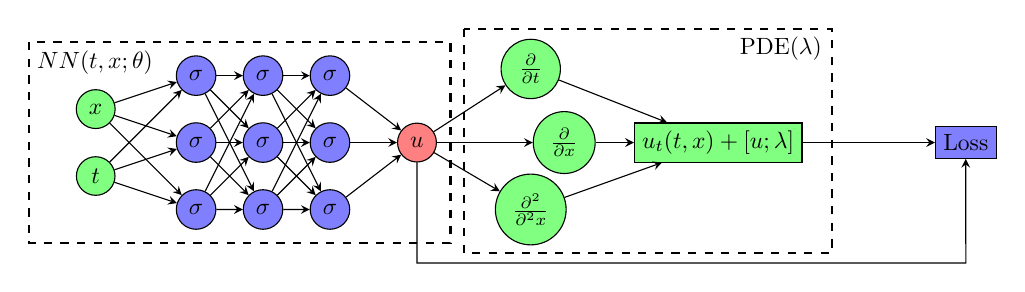
\begin{tikzpicture}[
      % Define styles
      neuron/.style={circle,draw,minimum size=.2cm},
      func/.style={rectangle,draw,minimum size=.2cm},
      PDE/.style={func, fill=green!50},
      loss/.style={func, fill=blue!50},
      input/.style={neuron, fill=green!50},
      hidden/.style={neuron, fill=blue!50},
      output/.style={neuron, fill=red!50},
      diff/.style={neuron, fill=green!50},
      arrow/.style={->,>=stealth},
      scale=0.85,
      transform shape
    ]
      
    \steporfull<3->{
      % Input Layer
      \draw[dashed, thick] (-1,0) rectangle (5.3,-3); % 前两个坐标为矩形左下角的坐标,后两个坐标为矩形右上角的坐标
      \node at (-1,0) [below right] {$NN(t,x; \theta)$}; % 文本内容为"文本",位置为方框的左上角

      \node[input] (Input0) at (0,-1) {$x$};
      \node[input] (Input) at (0,-2) {$t$};
    
      % Hidden Layer 1
      \node[hidden] (Hidden11) at (1.5,-0.5) {$\sigma$};
      \node[hidden] (Hidden12) at (1.5,-1.5) {$\sigma$};
      \node[hidden] (Hidden13) at (1.5,-2.5) {$\sigma$};
    
      % Hidden Layer 2
      \node[hidden] (Hidden21) at (2.5,-0.5) {$\sigma$};
      \node[hidden] (Hidden22) at (2.5,-1.5) {$\sigma$};
      \node[hidden] (Hidden23) at (2.5,-2.5) {$\sigma$};
    
      % Hidden Layer 3
      \node[hidden] (Hidden31) at (3.5,-0.5) {$\sigma$};
      \node[hidden] (Hidden32) at (3.5,-1.5) {$\sigma$};
      \node[hidden] (Hidden33) at (3.5,-2.5) {$\sigma$};

      % Output Layer
      \node[output] (Output) at (4.8,-1.5) {$u$};

      % Connect neurons Input-Hidden Layer 1
      \foreach \i in {1,2,3}
          \draw[arrow] (Input) -- (Hidden1\i);
        \foreach \i in {1,2,3}
          \draw[arrow] (Input0) -- (Hidden1\i);
    
      % Connect neurons Hidden Layer 1-Hidden Layer 2
      \foreach \i in {1,2,3}
          \foreach \j in {1,2,3}
              \draw[arrow] (Hidden1\i) -- (Hidden2\j);
    
      % Connect neurons Hidden Layer 2-Hidden Layer 3
      \foreach \i in {1,2,3}
          \foreach \j in {1,2,3}
              \draw[arrow] (Hidden2\i) -- (Hidden3\j);
    
      % Connect neurons Hidden Layer 3-Output
      \foreach \i in {1,2,3}
          \draw[arrow] (Hidden3\i) -- (Output);
    % }

    % \steporfull<2->{
      \draw[dashed, thick] (5.5,0.2) rectangle (11,-3.15);
      \node at (9.5,0.2) [below right] {PDE($\lambda$)}; % 文本内容为"文本",位置为方框的左上角
    %   % Partial Derivatives
      \node[diff] (D1) at (6.5,-0.4) {$\frac{\partial}{\partial t}$};
      \node[diff] (D2) at (7,-1.5) {$\frac{\partial}{\partial x}$};
      \node[diff] (D3) at (6.5,-2.5) {$\frac{\partial^2}{\partial^2 x}$};
      \node[PDE] (PDE) at (9.3,-1.5) {$u_t(t,x) + \varGamma \left[u; \lambda \right]$};

      \foreach \i in {1,2,3}
          \draw[arrow] (Output) -- (D\i);
      \foreach \i in {1,2,3}
          \draw[arrow] (D\i) -- (PDE);
    }

    % \steporfull<2->{
      \node[loss] (L) at (13,-1.5) {Loss};

      \draw[arrow] (Output) |- (13,-3.3) -- (L.south);
      \draw[arrow] (PDE.east) |- (L);
    % }
    \end{tikzpicture}
    \caption{PINN, with with 3 fully connected hidden layers}
    \label{}
\end{figure}
\end{frame}



\begin{frame}
  \frametitle{Introduction}
  \framesubtitle{Recap - Conclusion}
  \begin{block}{Comparing With Finite Difference Time Domain Method (FDTD)}
    \begin{enumerate}
      \item Deep Neural Network \cite{FIRST}
            \begin{itemize}
              \item Gives lower quality approximations.
              \item Takes longer time to train.
              \item Possible to solve high dimension PDEs \vspace*{1em}
            \end{itemize}
      \item Physics Informed Neural Network
            \begin{itemize}
              \item Gives higher quality approximations.
              \item Takes longer time to train.         
              \item Has more flexible way to get results.
              \item Possible to solve high dimension PDEs
            \end{itemize}
    \end{enumerate}    
  \end{block}
\end{frame}


% \subsection{Work Directions}
% \begin{frame}
%   \frametitle{Introduction}
%   \framesubtitle{Work Directions}
%   \begin{enumerate}
%     \item Implement FDTD and PINN in \texttt{C++/C}
%     \item Implement FDTD hybrid parallel version using \texttt{MPI/OpenMP}
%     \item Implement PINN GPU parallel version using \texttt{Libtorch/CUDA}
%     \item Performance optimization.
%     \item Running benchmarks
%   \end{enumerate}
% \end{frame}



\section{Problem Setups}

\subsection{General Form}
\begin{frame}
  \frametitle{General Form of problem}
  \begin{block}{}
    The PDE parametrized by number $\lambda$ and an operator $\mathcal{N}[\cdot; \lambda]$, 
    and assume the variable $x$ is a 2D or 3D spatio-vector which is written in 
    \begin{equation}
      \begin{cases}
        \displaystyle \frac{\partial u}{\partial t}\left(t,\vec{x}\right) + \mathcal{N}\left[u;\lambda\right] = 0 \\
        \displaystyle u\left(0,\vec{x}\right) = \varphi (\vec{x})
      \end{cases}
    \end{equation}
    where $\varphi$ is the initial condition, and $\vec{x}\in \Omega, t\in[0, +\infty)$.
  \end{block}


  \begin{block}{Boundary Conditions}
    The Dirichlet and Von Neurmann boundary conditions are formed as 
    \begin{equation}
      \begin{cases}
        \displaystyle u\left(t,\vec{x}\right) = g (t,\vec{x}) \\
        \displaystyle \frac{\partial u}{\partial \vec{n}} = g (t,\vec{x})  
      \end{cases}
    \end{equation}
    where $\vec{n}$ is the normal vector on $\overline{\Omega}$ the boundary of domain $\Omega$.
  \end{block}
\end{frame}


\subsection{Thermal Conduction Systems}
\begin{frame}
  \frametitle{Thermal Conduction Systems}
  \framesubtitle{Heat Equation 2D}
  \begin{block}{}
    The function 
    \begin{equation}
      u(t,x,y) = x + y - xy, \:\forall \alpha \in \mathbb{R}^1
    \end{equation}
    is the solution of 2D Heat Equation \ref{EQ:Heat2D} below
    \begin{align}\label{EQ:Heat2D}
      &\frac{\partial u}{\partial t} = \alpha \left(
        \frac{\partial u^2}{\partial^2 x}
        +
        \frac{\partial u^2}{\partial^2 y}
      \right) &(x,y) \in \Omega, \: t \in \left[0, +\infty\right)  \nonumber\\
      &u(0,x,y)  = \varphi(x,y) = 0 &(x,y) \in \Omega\\
      &u(t,x,y)
       = g(x,y)
       = \begin{cases}
        y, \:\: x=0, y\in\left(0,1\right)\\
        1, \:\: x=1, y\in\left(0,1\right)\\
        x, \:\: y=0, x\in\left(0,1\right)\\
        1, \:\: y =1, x\in\left(0,1\right)
      \end{cases}
      &t \in \left[0, +\infty\right) \nonumber
    \end{align}
  \end{block}
\end{frame}


\begin{frame}
  \frametitle{Thermal Conduction Systems}
  \framesubtitle{Heat Equation 3D}
  \vspace*{-0.3em}
  \begin{block}{}
    The function
    \begin{equation}
      u(t,x,y,z) = x + y + z - 2xy - 2xz - 2yz + 4xyz, \:\forall \alpha \in \mathbb{R}^1
    \end{equation}
    is the solution of 3D Heat Equation \ref{EQ:Heat3D} below
    \begin{align}\label{EQ:Heat3D}
      &\frac{\partial u}{\partial t} = \alpha \left(
        \frac{\partial u^2}{\partial^2 x}
        +
        \frac{\partial u^2}{\partial^2 y}
        +
        \frac{\partial u^2}{\partial^2 z}
      \right) & (x,y, z) \in \Omega, \: t \in \left[0, +\infty\right) 
                                                                      \nonumber\\
      &u(0,x,y,z)  = \varphi(x,y,z) = 0 &(x,y,z) \in \Omega\\
      &  u(t,x,y,z) = g(x,y,z) = 
      \begin{cases}
        y+z -2yz        , \:\: &x=0,\\
        1 - y - z + 2yz , \:\: &x=1,\\
        x+z - 2xz       , \:\: &y=0,\\
        1 - x - z + 2xz , \:\: &y =1,\\
        x+y - 2xy       , \:\: &z=0,\\
        1 - x - y + 2xy , \:\: &z=1
      \end{cases}
      &t \in \left[0, +\infty\right) \nonumber
    \end{align}
  \end{block}
\end{frame}

\section{Methodology}

\subsection{N-Dimension Matrix}
\begin{frame}
  \frametitle{N-dimension Matrix}
  \framesubtitle{STL containers}
  STL provides containers \texttt{std::array} and \texttt{std::vector} for creating one-dimension array.
  \\
  There are two way for dealing with high-dimension data:
  \begin{enumerate}
    \item Nesting the one dimension arrays or vectors.
    \item Hierarchy approach, designing derived classes of one-dimension array base class.
  \end{enumerate}
  \begin{figure}[htbp]
    \centering
    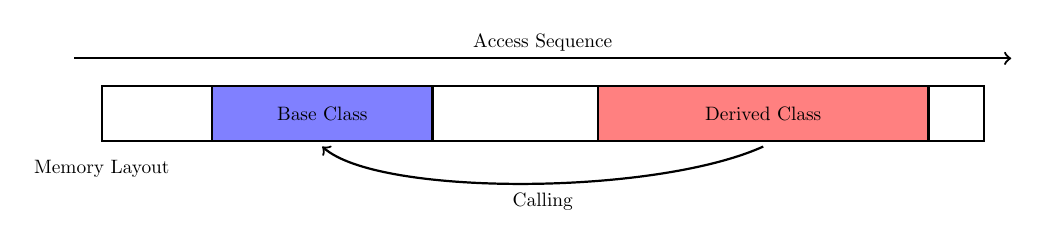
\begin{tikzpicture}[scale=0.7, transform shape]
      % \draw[help lines, step=1] (-10,-2) grid (10,2);    
      % % Draw axes
      % \draw[dashed,->] (-10,0) -- (10,0) node[right] {x};
      % \draw[dashed,->] (0,-2) -- (0,2) node[above] {y};

      \draw[thick, ->] (-8.5, 1.5) -- node[midway, above] {Access Sequence} (8.5, 1.5);

      \draw[thick] (-8,1) rectangle (8,0);
      \node at (-8,-0.5) [] {Memory Layout};

      \draw[thick, fill=blue!50] (-6,1) rectangle (-2,0);
      \node at (-4, 0.5) [] {Base Class};

      \draw[thick, fill=red!50] (1,1) rectangle (7,0);
      \node at (4, 0.5) [] {Derived Class};

      \node at (0, -1.1) [] {Calling};
      \draw[thick, ->] (4, -0.1) 
        .. controls (2, -1) and (-3, -1) .. (-4, -0.1);

    \end{tikzpicture}
    \caption{Derived Class calling members in Base class, timing is not predictable.}
    \label{<label>}
  \end{figure}
\end{frame}


\begin{frame}
  % \frametitle{N-dimension Matrix}
  % \framesubtitle{Memory Layout Problem}
  \begin{enumerate}
    \item Nesting multi-dimension array has non-contiguous memory layout.
    \item Derived class needs more time to access members in base class.
    \item Poor cache utilization leads to poor performance.
    \item MPI type create requires contiguous memory layout.
  \end{enumerate}
  % 插入图
  \begin{figure}[htbp]
    \centering
    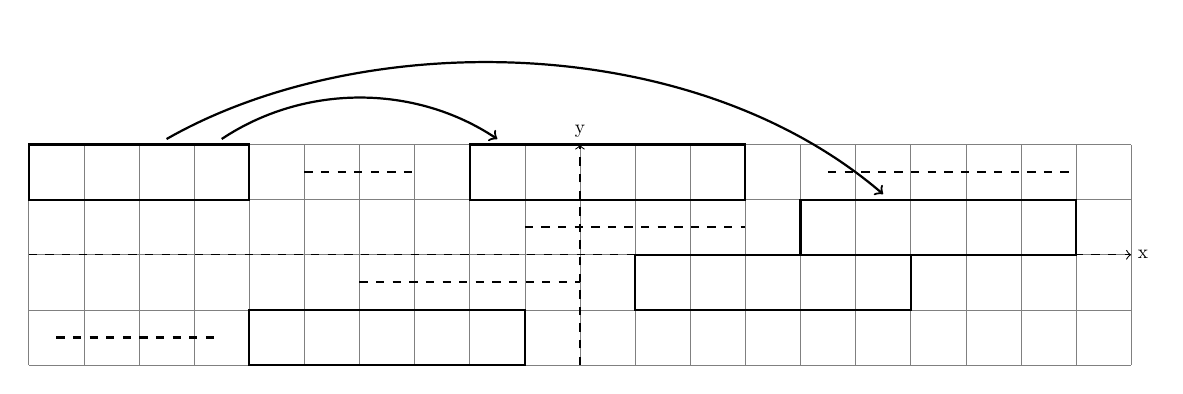
\begin{tikzpicture}[scale=0.7, transform shape]
      \draw[help lines, step=1] (-10,-2) grid (10,2);    
      % Draw axes
      \draw[dashed,->] (-10,0) -- (10,0) node[right] {x};
      \draw[dashed,->] (0,-2) -- (0,2) node[above] {y};

      \draw[thick] (-10,2) rectangle (-6,1);    
      \draw[dashed, thick] (-5,1.5) -- (-3, 1.5);

  
      \draw[thick] (-2,2) rectangle (3,1);
      \draw[dashed, thick] (4.5,1.5) -- (9, 1.5);

      \draw[dashed, thick] (-1,0.5) -- (3, 0.5);
      \draw[thick] (4,1) rectangle (9,0);
      

      \draw[thick] (1,0) rectangle (6,-1);
      \draw[dashed, thick] (-4, -0.5) -- (0, -0.5);

      \draw[dashed, thick] (-9.5, -1.5) -- (-6.5, -1.5);
      \draw[thick] (-6,-1) rectangle (-1,-2);


      \draw[thick, ->] (-6.5, 2.1) 
      .. controls (-5, 3.1) and (-3, 3.1) .. (-1.5, 2.1);

      \draw[thick, ->] (-7.5, 2.1) 
      .. controls (-4, 4.1) and (2, 4.1) .. (5.5, 1.1);
      
    \end{tikzpicture}
    \caption{<caption>}
    \label{<label>}
  \end{figure}
\end{frame}


\begin{frame}
  \frametitle{N-dimension Matrix}
  \framesubtitle{Solution}
  \begin{itemize}
    \item An external small \texttt{\_\_multi\_array\_shape} object defines the routines for accessing the elements.
    \item Smart pointer, ensure memory's contiguous layout and safety.
    \item Separate into two detail and user interface objects adhering RAII rules.
  \end{itemize}


  % 插入图
\end{frame}







\subsection{Parallelization of Multi-dimensional Matrices on cartesian Topologies}


% \section{Implementations}
% \subsection{PDE Solvers}
% % \subsection{General Setups}
% % \subsection{Parallel Strategies}


\subsection{PINN Model}

% \section{Related Work}
% \subsection{Finite Difference Time Domain Method}
% \subsection{Physics Informed Neural Network}


% \section{Problem Setups}
% \subsection{Continuous Form}
% \subsection{Discretization}


\section{Experiments}


\section{Discussion}



% \section{Introduction}
% % \subsection{Related Research}
% \begin{frame}
%   \frametitle{Introduction}
%   \framesubtitle{Related Researches}
%   \steporfull<1->{\begin{block}{Numerical Methods for Kolmogorov PDE}
%   \begin{itemize}
%     \item \steporfull<1->{Deterministic numerical approximation methods.} 
%     % (cf., \cite{brennan1978finite}\cite{brennan1977valuation}\cite{han2017overcoming}\cite{kloeden2012numerical})}
%     \item {Finite elements based approximation methods. }
%     % (cf., \cite{brenner2007mathematical}\cite{ciarlet2002basic}\cite{zienkiewicz1977finite})}
%     \item {Random numerical approximation methods based on Monte Carlo methods. }
%     % (cf., \cite{giles2008multilevel}\cite{graham2013stochastic})}
%   \end{itemize}
%   \end{block}}
%   \steporfull<2->{\begin{block}{Drawbacks}
%     \begin{itemize}
%       \item Curse of dimension.
%       \item Finite region.
%     \end{itemize}
%   \end{block}}
  
% \end{frame}

% % \subsection{Results}
% % \begin{frame}
% %   \frametitle{Introduction}
% %   \framesubtitle{Results}
% %   Approximate $u(T,x)$ at $x\in \left[a,b\right]^d$
% %   \vspace{1em}
% %   \begin{itemize}
% %     \item $x$ is vector in $\mathbb{R}^d$.
% %     \item $d$ is a large positive number.
% %     \item $x$ is in entire $\left[a,b\right]^d$. 
% %   \end{itemize}
% % \end{frame}



% \begin{frame}
%     \frametitle{Introduction}
%     \framesubtitle{Kolmogorove PDE}
%     \uncover{For $\mathbb{R}^1\owns T>0,\: x\in \mathbb{R}^d, t\in [0,T],\:u(t,x)=u \in \mathbb{R}^1$}
%     \vspace{1em}
%     \begin{block}{}
%       \vspace{0.5em}
%       \uncover{\begin{equation}
%         \frac{\partial u}{\partial t} = \frac{1}{2}
%         \Tr_{\mathbb{R}^d}\left[\sigma(x)\left[\sigma(x)\right]^*\Hess_x u\right] + 
%         \left< \mu(x), \nabla_xu \right>_{\mathbb{R}^d}
%       \end{equation}}
%     \end{block}
%     \uncover{
%       \begin{align}
%         &\mu(x) \in \mathbb{R}^d,\sigma(x)\in \mathbb{R}^{d\times d} \\
%         &u(0,x) = \phi(x)
%       \end{align}}
% \end{frame}

% \section{Algorithm}
% % \begin{frame}
% %   \frametitle{Algorithm}
% %   \framesubtitle{Framework}
% %   \begin{itemize}
% %     \item Transform PDE into SDE
% %     \item Determine function $u(T,x)$ equals to exception $\mathbb{E}\left[\phi(X_{t}^x)\right]$
% %     \item Equivalent to a minimization problem
% %     \item Discretization
% %     \item Deep Neural Network   
% %   \end{itemize}
% % \end{frame}
% \subsection{PDE to SED}
% \begin{frame}
%   \frametitle{Algorithm}
%   \framesubtitle{Transform PDE into SDE}
%   \begin{itemize}
%     \item Function $u(t,x)$ satisfies PDE \begin{equation*}
%       \frac{\partial u}{\partial t} = \frac{1}{2}
%       \Tr_{\mathbb{R}^d}\left[\sigma(x)\left[\sigma(x)\right]^*\Hess_x u\right] + 
%       \left< \mu(x), \nabla_xu \right>_{\mathbb{R}^d}
%     \end{equation*}
%     \item Stochastic Process 
%     $X_t^x$ satisfies SDE
%     \begin{equation}
%       \dis X_t^x = x + \int_{0}^{t}\mu(X^x_s)ds + \int_{0}^{t}\sigma(X_s^x)dW_s
%       \label{SDE}
%     \end{equation}
%     \item Feynman-Kac Formula: 
%     \begin{align}
%       % &\frac{\partial u(t,x)}{\partial t} + \Hess_x u(t,x) + \mu(x) u(t,x) = 0 \\
%       % &\phi(x) = u(0,x) \\
%       &u(t, x) = \mathbb{E}\left[ e^{ \dis -\int_t^T \mu(X_s^x) \, \dif s} \phi(X_T^x)  \right]
%     \end{align}
%     % \begin{equation}
%     %   \mathbb{E} \left[ \left( \int_{t}^{T} e^{\dis -\int_{t}^{t}V(X_s^x,s)\dif s} f(X_\tau^x,\tau)\dif \tau \right) + e^{\dis -\int_{t}^{T}V(X_\tau^x,\tau)  \dif \tau} \phi
%     %   (X_T^x) \right]
%     % \end{equation}
%     % \item Solution: \begin{equation}
%     %   u(T,x) = \mathbb{E}\left[ \phi \left( X_t^x \right)\right]
%     % \end{equation}
%   \end{itemize}


  


%   % \vspace{2em}
%   % \begin{columns}[T] % The [T] option aligns the column's content at the top

%   %   \begin{column}{.36\textwidth} % Left column and width
%   %     % Content of the left column
%   %     PDE
%   %     \begin{itemize}
%   %       \item Point A
%   %       \item Point B
%   %     \end{itemize}
%   %   \end{column}
%   %       % Add a vertical line here
%   %   \hspace*{.04\textwidth} % Spacing to push the line a bit right of the column
%   %   \vline{}
%   %   \begin{column}{.6\textwidth} % Right column and width
%   %     % Content of the right column
%   %     SDE
%   %     \begin{itemize}
%   %       \item $\dis X_t^x = x + \int_{0}^{t}\mu(X^x_s)ds + \int_{0}^{t}\sigma(X_s^x)dW_s$
%   %       \item $\mathbb{E}\left[\phi(X_{t}^x)\right]$
%   %     \end{itemize}
%   %   \end{column}

%   %   \end{columns}
% \end{frame}

% \begin{frame}
%   % \frametitle{Algorithm}
%   % \framesubtitle{Exception}
%   \begin{itemize}
%     \item With Stochastic Differential Equation:
%     \begin{equation*}
%       \dis X_t^x = x + \int_{0}^{t}\mu(X^x_s)ds + \int_{0}^{t}\sigma(X_s^x)dW_s 
%       % \label{SDE}
%     \end{equation*}
%     \vspace{1em}
%     \item Have the result:
%     \begin{align}
%       u(T,x) &= \mathbb{E}\left[ e^{ \dis -\int_T^T \mu(X_s^x) \, \dif s} \phi(X_T^x)  \right]\\
%           &= \mathbb{E}\left[ \phi \left( X_T^x \right)\right]
%     \end{align}
%     % \begin{equation}
%     %   u(T,x) = \mathbb{E}\left[ \phi \left( X_t^x \right)\right]
%     % \end{equation}
%   \end{itemize}
% \end{frame}

% \subsection{Minimization}
% % \begin{frame}
% %   \frametitle{Algorithm}
% %   \framesubtitle{Minimization}
% %   $u(T,x) = \mathbb{E}\left[ \phi \left( X_t^x \right)\right]$

% % \end{frame}
% \begin{frame}
%   \frametitle{Algorithm}
%   \framesubtitle{Minimization}
%   \steporfull<1->{\begin{block}{Proposition 2.7}
%     Stochastic process $X_t^x$ satisfies equation (\ref{SDE})\begin{equation*}
%       \dis X_t^x = x + \int_{0}^{t}\mu(X^x_s)ds + \int_{0}^{t}\sigma(X_s^x)dW_s
%     \end{equation*}
%     $x\in \mathbb{R}^d$ satisfies Kolmogorov PDE 
%   \end{block}}

%   \steporfull<2->{\begin{block}{Conclusion}
%     Unique $\exists U: [a,b]^d\rightarrow \mathbb{R}$, s.t.
%     \begin{equation}
%        \mathbb{E}\left[ \left| \phi(X_T^x) - U(\xi) \right|^2 \right] = \inf_{v \in C([a,b]^d,\mathbb{R})} \mathbb{E}\left[ \left| \phi(X_T^x) - v(\xi) \right|^2 \right]
%     \end{equation}
%     It holds that $U(x) = u(T,x)$, $\forall x\in [a,b]^d$.
%   \end{block}}
% \end{frame}

% % \begin{frame}
% %   \frametitle{Algorithm}
% %   \framesubtitle{Minimization}
% %   In order to find 
% %   \begin{equation*}
% %     u(T,x) = \mathbb{E}\left[\phi(X_{t}^x)\right]
% %   \end{equation*}
% %   \vspace{2em}

% %   Only determine the function $v$
% %   \begin{equation}
% %     v \in C\left(\left[a,b\right]^d,\mathbb{R}\right)
% %   \end{equation}
  
% %   To minimize 
% %   \begin{equation}
% %     \mathbb{E}\left[ \left| \phi(X_T^x) - v(\xi) \right|^2 \right]
% %   \end{equation}

% % \end{frame}
% \begin{frame}
%   \frametitle{Algorithm}
%   \framesubtitle{Minimization}
%   Extend 
%   \begin{equation*}
%     \mathbb{E}\left[ \phi \left( X_T^x \right)\right]
%   \end{equation*}
%   Minimize 
%   \begin{equation}
%     % \inf_{v \in C([a,b]^d,\mathbb{R})} 
%     \mathbb{E}\left[ \left| \phi(X_T^x) - v(x) \right|^2 \right] \,, v \in C\left([a,b]^d,\mathbb{R}\right)
%   \end{equation}
%   To get 
%   \begin{equation}
%     \mathbb{E}\left[ \left| \phi(X_T^x) - u(T,x) \right|^2 \right]
%     \label{minimization}
%   \end{equation}
%   % $\mathbb{E}\left[ \left| \phi(X_T^x) - u(T,x) \right|^2 \right] = \inf_{v \in C([a,b]^d,\mathbb{R})} \mathbb{E}\left[ \left| \phi(X_T^x) - v(x) \right|^2 \right]$
  

% \end{frame}


% \subsection{Discretization}
% \begin{frame}
%   \frametitle{Algorithm}
%   \framesubtitle{Discretization}
%   The Continues Stochastic Process
%   \begin{equation*}
%     \dis X_t^x = x + \int_{0}^{t}\mu(X^x_s)ds + \int_{0}^{t}\sigma(X_s^x)dW_s
%   \end{equation*}
%   Let
%   \begin{equation}
%     0=t_0 < t_1 < \dots < t_N = T
%   \end{equation}  
%   Discretized Stochastic Process of $\mathbb{X}_t^x$
%   \begin{equation}
%     \mathbb{X}_{t_{n+1}}^x = \mathbb{X}_{t_n}^x + \int_{t_n}^{t_{n+1}} \mu(\mathbb{X}_s^x) \, \dif s + \int_{t_n}^{t_{n+1}} \sigma(\mathbb{X}_s^x) \, \dif W_s
%   \end{equation}
% \end{frame}


% \begin{frame}
%   % Discretized Stochastic Process of $\mathbb{X}_t^x$
%   % \begin{equation*}
%   %   \mathbb{X}_{t_{n+1}}^x = \mathbb{X}_{t_n}^x + \int_{t_n}^{t_{n+1}} \mu(\mathbb{X}_s^x) \, \dif s + \int_{t_n}^{t_{n+1}} \sigma(\mathbb{X}_s^x) \, \dif W_s
%   % \end{equation*}
%   Approximate to 
%   \begin{equation}
%     \mathbb{X}_{t_{n+1}}^x \approx \mathbb{X}_{t_n}^x + (t_{n+1}-t_n) \mu(\mathbb{X}_s^x) + (t_{n+1}-t_n) \sigma(\mathbb{X}_s^x) 
%   \end{equation}
%   \vspace{1em}

%   Let a new Discretized Stochastic Process $\texttt{X}_n^x$ satisfies
%   \begin{equation}
%     \texttt{X}_{n+1}^x = \texttt{X}_{n}^x + (t_{n+1}-t_n) \mu(\texttt{X}_s^x) + (t_{n+1}-t_n) \sigma(\texttt{X}_s^x)   
%   \end{equation}
%   New minimization problem 
%   \begin{equation}
%     \mathbb{E}\left[ \left| \phi(X_T^x) - u(T,x) \right|^2 \right] 
%     \steporfull<2->{\longrightarrow 
%     \mathbb{E}\left[ \left| \phi(\texttt{X}_T^x) - u(T,x) \right|^2 \right]}
%     \label{new-minimization}
%   \end{equation}
% \end{frame}

% \begin{frame}
%   \frametitle{Algorithm}
%   \framesubtitle{Convergence}
%   \begin{block}{Theorem 2.8 (Strong Convergence)}
%     \vspace{0.5em}

%     There $\exists C \in (0,\infty)$ such that $\forall N \in \mathbb{N}$, holds that under $p$-norm
%     \begin{equation}
%       \sup_{n \in \{0,1,...,N\}} \left( E\left[ \left\| \mathbb{X}_{t_n^N}^x - \texttt{X}_n^N \right\|^p \right] \right)^{1/p} \leq C \left( \max_{n \in \{0,1,...,N-1\}} |t_{n+1} - t_n| \right)^{1/2}
%     \end{equation}

%     \vspace{1em}
%     \steporfull<2->{This means $\forall N \in \mathbb{N}$ holds that 
%     \begin{equation}
%       \lim_{N \to +\infty} \texttt{X}_{n}^{N} = \mathbb{X}_{t_{n}^N}^x = X_{T}^x
%     \end{equation}}
%     \vspace{0.5em}
%   \end{block}
% \end{frame}

% \subsection{Deep Neural Network}

% \begin{frame}
%   \frametitle{Algorithm}
%   \framesubtitle{Deep Neural Network (DNN)}
%   For Single Neuron, it takes $x\in \mathbb{R}^d$ as input, $A^{\theta}_{d,d}\in \mathbb{R}^{d\times d}$ and $b\in \mathbb{R}^d$ as parameters matrix.
%   \vspace{1em}

%   The output $y$ is 
%   \begin{equation}
%     y = \left[\begin{matrix}
%       A^{\theta}_{d,d} \mid b
%     \end{matrix} \right]
%     \left[\begin{matrix} x \\
%      1
%   \end{matrix}\right]
%   \end{equation}
% \begin{figure}[htbp]
%   \centering
%     \begin{tikzpicture}[
%       % Define styles
%       neuron/.style={circle, draw, fill=blue!20, minimum size=1cm},
%       arrow/.style={-Stealth},
%       output/.style={circle, draw, fill=green!20, minimum size=1cm} % 假设输出样式与神经元样式不同
%   ]

%       % Neuron
%       \node[neuron] (neuron) at (2,0) {Neuron};

%       % Input
%       \node[left=1cm of neuron] (input) {Input};
%       \draw[arrow] (input) -- (neuron);

%       % Output
%       \node[output] (output) at (5,0) {Output}; % 使用 output 样式
%       \draw[arrow] (neuron) -- (output);

%       % Activation Function
%       \draw[arrow] (output) -- (6.5,0) node[right] {Activation Function};

%   \end{tikzpicture}
%   \caption{Single Neuron Demonstration}
%   \label{<label>}
% \end{figure}
% \end{frame}

% \begin{frame}
%   \frametitle{Algorithm}
%   \framesubtitle{Deep Neural Network (DNN)}
%   Activation Function $L_d(x)$
%   \begin{align*}
%          & \sigmoid(x) = \frac{1}{1+e^{-x}}  \\ \\
%         % &= \left(\frac{1}{1+e^{-x_1}},\frac{1}{1+e^{-x_2}},\dots,\frac{1}{1+e^{-x_d}}\right) \\
%         &  \ReLU (x) = \max \{0,x\} \vspace{2em} \\ \\
%         &  \tanh (x) 
%   \end{align*}
% \end{frame}


% \begin{frame}
%   % \begin{figure}[htbp]
%   %   \centering
    
%   %   \includegraphics[width = 0.6\textwidth]{fig2.png}
%   %   \caption{Sigmoid Function when $x$ is 1 dimension}
%   %   \label{<label>}
%   % \end{figure}

%   \begin{figure}
%     \centering
%     % 第一个图像
%     \begin{minipage}{.33\textwidth}
%       \centering
%       \caption{$\sigmoid(x)$}
%     \includegraphics[width = \textwidth]{fig2.png}
%     % \caption{Sigmoid Function when $x$ is 1 dimension}
%     \end{minipage}%
%     \hfill
%     % 第二个图像
%     \begin{minipage}{.33\textwidth}
%       \centering
%       \caption{$\tanh (x)$}
%       \includegraphics[width = \textwidth]{fig2-1.png}
%       % \caption{Sigmoid Function when $x$ is 1 dimension}
%     \end{minipage}%
%     \hfill
%     % 第三个图像
%     \begin{minipage}{.33\textwidth}
%       \centering
%       \caption{$\ReLU (x)$}
%       \includegraphics[width = \textwidth]{fig2-2.png}
%     \end{minipage}
%     \caption{Activation Functions when $x$ is 1 dimension}
%   \end{figure}
% \end{frame}

% \begin{frame}
%   \frametitle{Algorithm}
%   \framesubtitle{Deep Neural Network (DNN)}
%   Architecture is Fully Connected Network
%   \begin{figure}[htbp]
%     \centering
%     \begin{tikzpicture}[
%       % Define styles
%       neuron/.style={circle,draw,minimum size=1cm},
%       input/.style={neuron, fill=green!50},
%       hidden/.style={neuron, fill=blue!50},
%       output/.style={neuron, fill=red!50},
%       arrow/.style={->,>=stealth}
%     ]
  
%     % Input Layer
%     \node[input] (Input) at (0,-2) {Input};
  
%     % Hidden Layer 1
%     \node[hidden] (Hidden11) at (2,0) {H1-1};
%     \node[hidden] (Hidden12) at (2,-2) {H1-2};
%     \node[hidden] (Hidden13) at (2,-4) {H1-3};
  
%     % Hidden Layer 2
%     \node[hidden] (Hidden21) at (4,0) {H2-1};
%     \node[hidden] (Hidden22) at (4,-2) {H2-2};
%     \node[hidden] (Hidden23) at (4,-4) {H2-3};
  
%     % Hidden Layer 3
%     \node[hidden] (Hidden31) at (6,0) {H3-1};
%     \node[hidden] (Hidden32) at (6,-2) {H3-2};
%     \node[hidden] (Hidden33) at (6,-4) {H3-3};
  
%     % Output Layer
%     \node[output] (Output) at (8,-2) {Output};
  
%     % Connect neurons Input-Hidden Layer 1
%     \foreach \i in {1,2,3}
%         \draw[arrow] (Input) -- (Hidden1\i);
  
%     % Connect neurons Hidden Layer 1-Hidden Layer 2
%     \foreach \i in {1,2,3}
%         \foreach \j in {1,2,3}
%             \draw[arrow] (Hidden1\i) -- (Hidden2\j);
  
%     % Connect neurons Hidden Layer 2-Hidden Layer 3
%     \foreach \i in {1,2,3}
%         \foreach \j in {1,2,3}
%             \draw[arrow] (Hidden2\i) -- (Hidden3\j);
  
%     % Connect neurons Hidden Layer 3-Output
%     \foreach \i in {1,2,3}
%         \draw[arrow] (Hidden3\i) -- (Output);
  
%     \end{tikzpicture}
%     \caption{FCN with 4 layers (3 hidden layers)}
%     \label{<label>}
% \end{figure}
% \end{frame}


% \begin{frame}
%   \frametitle{Algorithm}
%   \framesubtitle{Architecture of DNN}
%   \begin{itemize}
%     % \item Parameters are $\theta$
%     % \item Architecture is Fully Connected Network (FCN) with $s$ layers.
%     % \item Activation function $L$ is 
%     % \begin{equation}
%     %   L_d(x) = \frac{1}{1+e^{-x}}
%     % \end{equation}
%     \item Equation of model with $s$ layers
%     \begin{equation}
%       \mathbb{U}(\theta, x) = \left[ \left(A^{\theta,(s-1)d(d+1)}_{d,1} \circ L_d\right) \dots  \left(\circ A^{\theta,d(d+1)}_{d,d}  \circ L_d\right) \circ A^{\theta,0}_{d,d} \right] (x)
%     \end{equation}
%     \item Approximation method represented as 
%     \begin{equation}
%       \mathbb{U}(\theta, x) \approx u(T,x)
%     \end{equation}

%   \end{itemize}
% \end{frame}

% \begin{frame}
%   \frametitle{Algorithm}
%   \framesubtitle{Framework }
%   \begin{itemize}
%     \item Transform PDE to get SDE: $\dis X_t^x = x + \int_{0}^{t}\mu(X^x_s)ds + \int_{0}^{t}\sigma(X_s^x)dW_s $
%     \item Determine $u(T,x) = \mathbb{E}\left[\phi(X_{t}^x)\right]$
%     \item Equivalent to a minimization problem $\mathbb{E}\left[ \left| \phi(X_T^x) - v(\xi) \right|^2 \right]$
%     \item Discretize $X_t^{x}$ to get $\texttt{X}_n^N$
%     \item Deep Neural Network to get $\mathbb{U}(\theta,x) \approx U(T,x)$ 
%   \end{itemize}
% \end{frame}



% \section{Examples}
% \begin{frame}
%   \frametitle{Examples}
%   \begin{itemize}
%     \item Heat Equation
%     \begin{equation}
%       \frac{\partial u(t,x) }{\partial t} = \Delta_x u(t,x)
%     \end{equation}
%     \item Stochastic Lorenz Equation
%     \begin{equation}
%       \begin{aligned}
%       \left( \frac{\partial u}{\partial t} \right)(t, x) &= \frac{\beta^2}{2} (\Delta_x u)(t, x)
%        + \alpha_1(x_2 - x_1)\left( \frac{\partial u}{\partial x_1} \right)(t, x) \\
%       &\quad + (\alpha_2 x_1 - x_2 - x_1 x_3)\left( \frac{\partial u}{\partial x_2} \right)(t, x) \\
%       &\quad + (x_1 x_2 - \alpha_3 x_3)\left( \frac{\partial u}{\partial x_3} \right)(t, x).
%       \end{aligned}
%       \end{equation}
%   \end{itemize}
% \end{frame}

% \begin{frame}
%   \begin{itemize}
%     \item Heston Model
%     \begin{equation}
%       \begin{aligned}
%       &\left( 
%         \frac{\partial u}{\partial t} 
%       \right)(t, x) 
%       = \sum_{i=1}^{\delta} 
%           \left[ 
%             \alpha x_{2i-1} 
%             \left( 
%               \frac{\partial u}{\partial x_{2i-1}} 
%             \right)(t, x) 
%           + \kappa(\theta - x_{2i}) 
%             \left( 
%               \frac{\partial u}{\partial x_{2i}} 
%             \right)(t, x) 
%           \right] \\
%       & + \sum_{i=1}^{\delta} 
%       \left[
%         \frac{|x_{2i}|}{2} 
%         \left( 
%             |x_{2i-1}|^2 \left( \frac{\partial^2 u}{\partial x_{2i-1}^2} \right)(t, x) 
%           + 2x_{2i-1}\beta\rho \left( \frac{\partial^2 u}{\partial x_{2i-1} \partial x_{2i}} \right)(t, x)
%         \right)
%       \right] \\
%       & + \sum_{i=1}^{\delta} |x_{2i-1}|^2\beta^2 \left( \frac{\partial^2 u}{\partial x_{2i}^2} \right)(t, x) 
%       \end{aligned}
%     \end{equation}
%   \end{itemize}
% \end{frame}



% \begin{frame}
%   \frametitle{Heat Equation}
%   \framesubtitle{Solution}
%   For $x \in \mathbb{R}^d$, $t\in [0,T]$
%   \begin{equation}
%     \frac{\partial u(t,x) }{\partial t} = \Delta_x u(t,x)
%   \end{equation}
%   Solution
%   \begin{equation}
%     u(t,x) = ||x||^2_{\mathbb{R}^d} + td
%   \end{equation}
% \end{frame}

% \begin{frame}
%   \frametitle{Heat Equation}
%   \framesubtitle{Hyperparameters}
%   \begin{itemize}
%     \item Adam Optimizer
%     \item Learning Rate $10^{-3}$
%     \item  Loss function (Equation \ref{new-minimization})
%     \begin{equation}
%       l(\Theta_m) = \mathbb{E}\left[ |\phi(\texttt{X}_N^x) - \mathbb{U}(\Theta_m,x)|^2 \right]
%     \end{equation}
%     \item Batch size 8192
%   \end{itemize}

  

% \end{frame}
% \begin{frame}
%   \frametitle{Heat Equation}
%   \framesubtitle{Relative error}
%   Calculate Relative Errors 
%   % \begin{equation}
%   %   \int_{[0,1]^d} \left| \nu(T, x) - U_{\Theta_m,1,S_m}(x) \right| \, dx
%   % \end{equation}
%   % \begin{equation}
%   %   \left( \int_{[0,1]^d} \left| \nu(T, x) - U_{\Theta_m,1,S_m}(x) \right|^2 \, dx \right)^{1/2}
%   % \end{equation}
%   % \begin{equation}
%   %   \sup_{x \in [0,1]^d} \left| \nu(T, x) - U_{\Theta_m,1,S_m}(x) \right|
%   % \end{equation}
    
    
    
%   \begin{align}
%     L^1\left(\lambda_{[0,1]^{d}} ; \mathbb{R}\right) &= \int_{[0,1]^d} \left| u(T, x) - \mathbb{U}(x,\Theta_m) \right| \, \dif x \\
%     L^2\left(\lambda_{[0,1]^{d}}; \mathbb{R}\right) &=\sqrt{ \int_{[0,1]^d} \left| u(T, x) - \mathbb{U}(x,\Theta_m) \right|^2 \, \dif x } \\
%     L^{\infty}\left(\lambda_{[0,1]^{d}}; \mathbb{R}\right) &=\sup_{x \in [0,1]^d} \left| \frac{u(T, x) -\mathbb{U}(x,\Theta_m)}{u(T,x)} \right|
%   \end{align}
% \end{frame}

% \begin{frame}
%   \frametitle{Relative Approximation Errors}
%   % \framesubtitle{Heat Equation}
%   \begin{figure}
%   \centering
%   \includegraphics[width=0.8\linewidth]{Screenshot 2023-11-10 at 10.30.47.png}% Adjust the size as needed
%   \caption{Image caption (adapted from Author, Year)}
%   \label{fig:image_label}
%   \end{figure}

% \end{frame}

% \begin{frame}
%   \frametitle{Relative Approximation Errors}
%   \framesubtitle{Heat Equation}
%   % 使用resizebox来调整表格到幻灯片宽度
%   \begin{table}[ht]
%   \scriptsize
%   \resizebox{\textwidth}{!}{%
%   \begin{tabular}{@{}p{1.2cm}|p{2.1cm}|p{2.1cm}|p{2.1cm}|p{1.2cm}@{}}
%   \toprule
%   Number of steps & Relative \(L^1(\lambda_{[0,1]^d}; \mathbb{R}) \)-error & Relative \( L^2(\lambda_{[0,1]^d}; \mathbb{R}) \)-error & Relative \( L^\infty(\lambda_{[0,1]^d}; \mathbb{R}) \)-error & Mean runtime in seconds \\ \midrule
%   0 & 0.998253 & 0.998254 & 1.003524 & 0.5 \\
%   10000 & 0.957464 & 0.957536 & 0.993083 & 44.6 \\
%   50000 & 0.786743 & 0.786806 & 0.828184 & 220.8 \\
%   100000 & 0.574013 & 0.574060 & 0.605283 & 440.8 \\
%   150000 & 0.361564 & 0.361594 & 0.384105 & 661.0 \\
%   200000 & 0.150346 & 0.150362 & 0.164140 & 880.8 \\
%   500000 & 0.000882 & 0.001112 & 0.007360 & 2200.7 \\
%   750000 & 0.000822 & 0.001036 & 0.007423 & 3300.6 \\
%   \bottomrule
%   \end{tabular}%
%   }
%   \caption{Approximate presentations of the relative approximation errors}
% \label{your_label_here}
% \end{table}
% \end{frame}




% % \begin{frame}
% %   \frametitle{Table of Contents}
% %   \tableofcontents
% % \end{frame}

% % \section{Introduction}
% % \begin{frame}
% %   \frametitle{Introduction}
% %   % Add your introduction content here
% % \end{frame}

% % \section{Theoretical Framework and Assumptions}
% % \begin{frame}
% %   \frametitle{Theoretical Framework and Assumptions}
% %   % Add content about theoretical framework and assumptions here
% % \end{frame}

% % \section{Key Algorithms and Methods}
% % \begin{frame}
% %   \frametitle{Key Algorithms and Methods}
% %   % Add content about algorithms and methods here
% % \end{frame}

% % \section{Numerical Simulations and Python Code}
% % \begin{frame}
% %   \frametitle{Numerical Simulations and Python Code}
% %   % Add content about numerical simulations and Python code here
% % \end{frame}

% % \section{Error Calculation and Analysis}
% % \begin{frame}
% %   \frametitle{Error Calculation and Analysis}
% %   % Add content about error calculation and analysis here
% % \end{frame}

% % \section{Case Studies and Practical Applications}
% % \begin{frame}
% %   \frametitle{Case Studies and Practical Applications}
% %   % Add content about case studies and practical applications here
% % \end{frame}

% \section{Conclusion}
% \begin{frame}
%   \frametitle{Conclusion}
%   Propose an algorithm to approximate Kolmogorov PDE

%   which aims to overcome:\vspace{1em}
%   \begin{itemize}
%     \item Curse of Dimensionality\vspace{1em}
%     \item Finite Region\vspace{1em}
%   \end{itemize}
% \end{frame}

% \section{Future Research Directions}
% \begin{frame}
%   \frametitle{Future Research Directions}
%   \begin{itemize}
%     \item \steporfull<1-> {Reproduce the Algorithm\vspace{1em}}
%     \item \steporfull<2-> {Compare to Exited Numerical Method \vspace{1em}}
%     \item \steporfull<3-> {Conditioning \& Sensitivity \vspace{1em}}
%     \item \steporfull<4-> {Different Structure\vspace{1em}}
%     \item \steporfull<5-> {Different Training Strategy\vspace{1em}}
%   \end{itemize}
  

% \end{frame}

\begin{frame}
  \frametitle{Closing Remarks}
  \centering
  {\Large Thank you for your attention!}\\
  \vspace{2em}
  {\large Any questions?}
\end{frame}


% \begin{frame}[allowframebreaks]
%   \frametitle{References}
%   \printbibliography
% \end{frame}

\end{document}

